\documentclass[12pt]{article}
\usepackage{amssymb,amsfonts,amsmath,graphicx,mathtools}
\usepackage[alphabetic,y2k,lite]{amsrefs}
\usepackage{fullpage, mystyle}
\usepackage{MnSymbol}

\usepackage{tikz}
\usepackage{tikz-cd}


\newcommand{\cB}{{\mathcal{B}}}
\newcommand{\cD}{{\mathcal{D}}}
\newcommand{\Mod}{{\mathcal{M}od}}
\newcommand{\cHom}{{\mathcal{H}\text{om}}}
\newcommand{\mmod}{{\textrm{mod}}}
\newcommand{\cFun}{{\mathcal{F}un}}
\newcommand{\Vect}{{\textrm{Vec}}}

\newcommand{\bigboxplus}{\Huge \boxplus}%{{\scalebox{2}{\boxplus}}}

\begin{document}

\title{Note in preparation for talk for seminar on Fusion 2-Categories, Winter semester 2022, UHH}
\author{Ying Hong Tham}
\date{28 December, 2022}
\maketitle

[Almost everything here is from \cite{DRfusion};
the only things that are new here are
cleaner proofs of the main theorems]


The main goal of my talk today is to prove that
a finite semisimple 2-category is the
category of finite semisimple modules
over a multifusion category,
and vice versa.


That is, for a semisimple 2-category $\cC$,
there exists a multifusion category $C$
such that

\[
\cC \simeq \Mod_{s.s.}^{fin}(C)
\]

Here $\Mod_{s.s.}^{fin}(C)$,
which we will abbreviate to $\Mod-C$,
stands for finite semisimple right module categories over $C$.

Conversely, for any mutifusion category $C$,
$\Mod-C$ is a semisimple 2-category.



\subsection{Conventions}

Everything is over an algebraically closed field $\kk$
with characteristic 0.

We use different fonts/alphabets for different levels
of structures:

In relation to a 2-category:
\begin{itemize}
\item $\cC$ (caligraphic font): 2-category;

\item $X,Y,F$ (upper case latin): object of 2-category,
	functor between 2-categories;

\item $f,g$ (lower case latin): 1-morphism;
	we write $\cC(X,Y)$ for the category of morphisms
	from $X$ to $Y$;

\item $\eta,\veps,\delta$ (lower case greek): 2-morphism;
	for a 2-morphism $\alpha: f \Rightarrow g: X \to Y$,
	we may write $\alpha \in \cC(X,Y)(f,g)$
	to indicate its sources and targets,
	or simply $\alpha \in \Hom(f,g)$ if the objects are clear
\end{itemize}

In relation to a 1-category:
\begin{itemize}
\item $C,A$ (upper case latin): category;

\item $a,b,f,g$ (lower case latin): objects in category,
	functor between categories;

\item $\alpha,\beta$ (lower case greek): morphism in category
\end{itemize}

[We use the same type of font for 1-functors and 1-morphisms
because the 1-morphisms in the 2-category $\Mod(C)$
of module categories are module functors,
and we want the notation to be consistent;
we use the same type of font for 2-functors and objects
because 2-functors are objects in the 2-category of
2-functors]

We also compose morphisms from right to left:
in a 2-category $\cC$,
for $\alpha \in \cC(X,Y)(f,f'),
\beta \in \cC(Y,Z)(g,g'),
\gamma \in \cC(X,Y)(f',f'')$,
we write
\[
g \circ f, g \circ f', \ldots : X \to Z
\]
for composition of 1-morphisms,
\[
\beta \circ \alpha: (g \circ f) \Rightarrow (g' \circ f'):
	X \to Z
\]
for horizontal composition of 2-morphisms,
\[
\gamma \cdot \alpha: f \Rightarrow f'' : X \to Y
\]
for vertical composition of 2-morphisms.


We may also omit the composition symbols
if the type of composition is clear
(in particular for composition of 1-morphisms).



In general, if $P$ is a property of a 1-category,
we say that a 2-category $\cC$ is \emph{locally $P$}
if every hom-category $\cC(X,Y)$ satisfies $P$.


By 2-category we always mean a weak 2-category
that is furthermore locally additive over $\kk$,
that is, all hom-categories are
additive categories over $\kk$,
and all compositions are $\kk$-bilinear.
By 2-functor (sometimes just functor for simplicity)
between 2-categories will always be locally $\kk$-linear.


\section{Review}

Let us recall some definitions and facts concerning
semisimple 2-categories.
These where covered in more detail in previous talks,
so here we will simply state them without proof.

\subsection{Additive 2-category, direct sums of objects}

\begin{definition}[direct sum of objects in 2-category]
A \emph{direct sum} of two objects $A_1,A_2$ in $\cC$
is an object $A_1 \boxplus A_2$ together with
inclusion and projection 1-morphisms
$i_k : A_k \rightleftharpoons A_1 \boxplus A_2 : p_k$,
such that
\begin{itemize}
\item $p_k \circ i_k \simeq \id_{A_k}$,
\item $p_2 \circ i_1$, $p_1 \circ i_2$ are zero 1-morphisms,
\item $\id_{A_1 \boxplus A_2} \simeq
	i_1 \circ p_1 \oplus i_2 \circ p_2$
\end{itemize}
\end{definition}

\begin{proposition}
$i_k,p_k$ are two-sided adjoints to each other.
\end{proposition}


\begin{definition}
A 1-morphism $i: X \to Y$ is \emph{fully faithful}
(or $(X,i)$ is a \emph{subobject} of $Y$)
if it induces fully faithful functors between hom-categories
by post-composition, i.e. for all objects $A$,
$i \circ - : \cC(A,X) \to \cC(A,Y)$
is fully faithful.
\end{definition}

\begin{proposition}
$i_k: A_k \to A_1 \boxplus A_2$ is fully faithful.
\end{proposition}



(I don't think the following was discussed,
but it is a simple concept anyway)

\begin{definition}[Direct sum of 2-categories]
Given 2-categories $\cC_j$, $j \in J$,
we may consider the direct sum 2-category
$\cC := \bigboxplus_{j \in J} \cC_j$:
\begin{itemize}
\item $\Obj \cC = \bigsqcup_{j \in J} \Obj \cC_j$

\item for $X \in \cC_i, Y \in \cC_j$,
	$\cC(X,Y) =
\begin{cases}
	\cC_j(X,Y) \;\; \text{if } i = j
	\\
	0 \;\; \text{if } i \neq j
\end{cases}
$
\end{itemize}
\end{definition}

\subsection{Idempotent completeness, separable monads, splittings}

\begin{definition}
Let $(t, \mu, \eta)$ be a monad on an object $X$
in a 2-category $\cC$.
We say $t$ is \emph{separable} if there is a
$t$-$t$-bimodule section
$\delta: t \Rightarrow t \circ t$ to $\mu$.
\end{definition}

\begin{definition}
Let $r \vdash l: X \to Y$ be an adjunction
with unit $\eta: \id_X \Rightarrow rl$
and counit $\veps: lr \Rightarrow \id_Y$.
We say the adjunction $l \dashv r$ is \emph{separable}
if $\veps$ admits a section.
\end{definition}

Clearly, if an adjunction $l \dashv r$ is separable,
then the monad $rl$ is separable.

\begin{definition}
Let $(t,\mu,\eta)$ be a separable monad on
an object $X \in \cC$.
A \emph{(separable) splitting} of $t$ is a (separable) adjunction
$r \vdash l: X \to Y$
together with an isomorphism
$\psi: rl \simeq t$ as monads on $X$.
\end{definition}

Under the right conditions
(local idempotent completeness of $\cC$),
separable splittings are unique:


\begin{proposition}[Uniqueness of separable splitting]
[\cite{DRfusion}*{Theorem A.3.1}]
\label{p:splitting-unique}
In a locally idempotent complete 2-category $\cC$,
separable splittings of a separable monad are unique
up to equivalence.
\end{proposition}

In particular, this holds true when $\cC$
is locally semisimple.

Thought to self:
\cite{DRfusion} proves this by showing that
a splitting is equivalent
to an ``Eilenberg-Moore object'' and also a ``Kleisli object'',
which are in themselves important and interesting objects
characterized by universal properties.
I'd like to have a more direct proof,
somehow constructing an equivalence between any two splittings
directly from the splitting data.
I don't have a full proof, but here's an attempt.
Say for a separable monad $t$ on $X$,
we have two adjunctions $r \vdash l : X \to Y$
and $r' \vdash l' : X \to Y'$
that split $t$.
There is are obvious 1-morphisms $l' \circ r: Y \to Y'$,
$l \circ r': Y' \to Y$,
but it is unlikely that these are equivalences.
A promising candidate for an equivalence
is $l' \circ_t r$, the coequalizer of
$l' \circ t \circ r \Rightarrow l' \circ r$
(here $r$ is a left $t$-module from the counit:
$tr \simeq rlr \Rightarrow r$;
similarly $l'$ is a right $t$-module).
Such a coequalizer does appear in the proof of
\cite{DRfusion}*{Theorem A.3.1} anyway,
and I've found that this thought process
makes the consideration of the Eilenberg-Moore and Kleisli
objects more motivated.


Now that we've defined the notion on objects,
we consider the property as a global 2-category-wide property:


\begin{definition}
A 2-category $\cC$ is \emph{idempotent complete}
if every separable monad admits a splitting.
\end{definition}

\begin{definition}
Let $\cC$ be a locally semisimple
(more generally locally idempotent complete)
2-category.
Define the \emph{idempotent completion of $\cC$},
denoted $\cC^\nabla$, to be the 2-category whose objects
are given by separable monads of $\cC$,
and the hom-category of morphisms from
separable monad $(X,p)$ to $(Y,q)$
is the category $q$-mod-$p(\cC(X,Y))$
of $q$-$p$-bimodules in $\cC(X,Y)$.

There is a natural 2-functor $I: \cC \to \cC^\nabla$
that is fully faithful.

A 2-functor $F: \cC \to \cD$
extends to a 2-functor $F^\nabla: \cC^\nabla \to \cD^\nabla$
that commutes with $I$'s.
\end{definition}

This is a categorified version of the Karoubi completion
operation.
By going along the lines of \cite{Ostrik},
the definition of $\cC^\nabla$
is very suggestive of the idea that
objects of $\cC^\nabla$ should be thought of as
the Morita 2-category of algebras in some tensor category;
indeed, this will be made precise in the proof
of the main result.


We can already the essence of this idea in the simple
example below.
Let $C$ be multifusion,
and let $\cB C$ be the 2-category with one object $*$
and endmorphisms given by $C$.
Then by construction, we have
\[
(\cB C)^\nabla =
\begin{cases}
	\Obj: \text{ separable algebras in } C
	\\
	\text{Mor}: (\cB C)^\nabla (a,b) = b\text{-bimod-}a(C)
\end{cases}
\]



\begin{proposition}
$\cC^\nabla$ is idempotent complete.
Moreover, if $\cC$ is already idempotent complete,
then $I: \cC \simeq \cC^\nabla$ is an equivalence.
\end{proposition}

As a consequence, if $\cD$ is idempotent complete,
then we have equivalences of 2-categories
\[
\cFun(\cC,\cD) \simeq \cFun(\cC^\nabla,\cD^\nabla)
\simeq \cFun(\cC^\nabla, \cD)
\]



\subsection{Simple objects}


\begin{proposition}[equivalent notions of simple-ness]
Let $\cC$ be a locally finite semisimple and
idempotent complete 2-category,
and let $X \in \cC$ be a nonzero object.
Then the following notions of $X$ being simple are equivalent:

(1) any subobject $i: Y \to X$ of $X$
 is either 0 ($Y \simeq 0$)
 or ($i$ is) an equivalence;

(2) $X$ cannot be written as a non-trivial direct sum,
	i.e. if $X = \boxplus X_i$,
	then $X_i \simeq 0$ for all but one $i$;

(3) $\id_X$ is a simple object in $\cC(X,X)$.
\end{proposition}

\begin{proof}[Proof idea]
(1) $\Rightarrow$ (2): Contravariant statement
follows from fully faithfulness of
$i_k: A_k \to A_1 \boxplus A_2$.

(2) $\Rightarrow$ (3): Contravariant statement is
``identity splitting implies object splitting'',
uses idempotent completeness of $\cC$
to split out objects corresponding to summands of $\id_X$
(which are separable monads)
(see \cite{DRfusion}*{Prop 1.3.16}).

(3) $\Rightarrow$ (1): for non-zero fully faithful $r: Y \to X$,
with $\id_X$ simple,
consider the left adjoint $l: X \to Y$,
use fully faithfulness to get a preimage
$\delta : \id_Y \Rightarrow lr$ of
$\eta \circ r: r \Rightarrow rlr$.
Use simplicity of $\id_X$ to get section of the unit $\eta$.
Show $\delta$ is a section of the counit. Etc.
(See \cite{DRfusion}*{Prop 1.2.14})
\end{proof}


\subsection{Semisimple 2-category}


\begin{definition}[(finite) semisimple 2-category]
A 2-category $\cC$ is \emph{semisimple}
if it is:
\begin{itemize}
\item locally semisimple,
\item admits left and right adjoints for every 1-morphism,
\item additive,
\item idempotent complete.
\end{itemize}

It is furthermore \emph{finite semisimple}
if it is also locally finite and
has finitely many equivalence classes of simple objects.
\end{definition}



%%%%%%%%%%%%%%%%%%%%%%%%%%%%%%%%%%%%%%%%%%%%%%%%%%%%%%%%%%%%%%
\section{New stuff}

Beyond this point, we cover new stuff.
Thus, the writing will be more speech like,
and written to reflect more or less the order of presentation
during the talk (at least how I plan to present it).


\subsection{Schur's lemma}

The equivalence between notions of a simple object
in a seimsimple 2-category,
as we just recalled,
is quite similar to the semisimple 1-category case.
However, there is a stark difference in that
there can be nonzero morphisms between
non-equivalent simple objects;
indeed, recall our running example of a 2-category
$\Mod(\Vect_{\ZZ/2})$:

\[
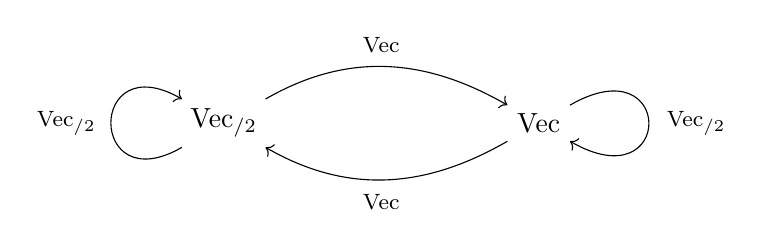
\begin{tikzpicture}
\node (a) at (0,0) {$\Vect_{\ZZ/2}$};
\node (b) at (4,0) {$\Vect$};
\draw[->] (a) to[out=30,in=150] (b);
\node at (2,1) {\footnotesize $\Vect$};
\draw[->] (b) to[out=-150,in=-30] (a);
\node at (2,-1) {\footnotesize $\Vect$};
\draw[->] (a) .. controls +(-150:2cm) and +(150:2cm) .. (a);
\node at (-2,0) {\footnotesize $\Vect_{\ZZ/2}$};
\draw[->] (b) .. controls +(30:2cm) and +(-30:2cm) .. (b);
\node at (6,0) {\footnotesize $\Vect_{\ZZ/2}$};
\end{tikzpicture}
\]


The existence of nonzero 1-morphisms
between non-equivalent simple objects
turns out to be a very important aspect of semisimple 2-categories
since, as we shall see,
it captures 2-Morita equivalences between fusion categories.

\begin{proposition}
[Schur's Lemma, \cite{DRfusion}*{Prop 1.2.19}]
\label{p:schur-lemma}
In a semisimple 2-category $\cC$,
if $f: A \to B, g: B \to C$ are nonzero 1-morphisms
between simple objects $A,B,C$,
then $g \circ f$ is also nonzero.
\end{proposition}

\begin{proof}[Proof of \prpref{p:schur-lemma}]
Let $f^*: B \to A$ be a right adjoint to $f$.
Since $\id_B$ is simple, there exists a section
$\delta: \id_B \Rightarrow ff^*$
to the counit $\veps: ff^* \Rightarrow \id_B$.
Postcomposing with $g$,
we have $\id_g = (\id_g \circ \veps) \cdot (\id_g \circ \delta):
g \Rightarrow gff^* \Rightarrow g$.
Thus if $gf = 0$, then $\id_g = 0$,
contradicting nonzero-ness of $B$.
\end{proof}

Thus, this establishes transitivity on a weaker notion
of equivalence among simple objects
(namely, existence of nonzero 1-morphism);
reflexivity is obvious,
and symmetry is given by adjoints.

\begin{definition}[component of semisimple 2-category]
In a semisimple 2-category $\cC$,
we say two simple objects $A,B$ belong to the same
\emph{component} if there exists a nonzero 1-morphism
$f: A \to B$.
\end{definition}


In a finite semisimple 2-category $\cC$,
there will be finitely many components,
say index by a set $J$.
Consider one component $j \in J$,
and consider the full subcategory $\cC_j$ of $\cC$
consisting of objects that are equivalent
to a direct sum of simples in the component $j$.
Clearly, this gives us a decomposition of $\cC$ into a direct sum
$\cC \simeq \bigboxplus_{j \in J} \cC_j$.


\subsection{Main result}

\begin{theorem}[\cite{DRfusion}*{Theorem 1.4.8}]
The 2-category of finite semisimple module categories
of a multifusion category
is a finite semisimple 2-category.
\end{theorem}

\begin{proof}
Let $C$ be a multifusion category.

Hmm see Prop 1.3.13, should I put that in the discussion
of idempotent completion?
\end{proof}


\begin{theorem}[\cite{DRfusion}*{Theorem 1.4.9}]
Every finite semisimple 2-category is equivalent to
the 2-category of finite semisimple module categories
of a multifusion category.
\end{theorem}

\begin{proof}
\end{proof}


\begin{thebibliography}{1}

\bibitem{DRfusion} Douglas, Christopher L., and David J. Reutter. ``Fusion
2-categories and a state-sum invariant for 4-manifolds.'' arXiv preprint arXiv:1812.11933 (2018).

\bibitem{Ostrik} Ostrik, Victor. ``Module categories, weak Hopf algebras and
modular invariants.'' Transformation groups 8, no. 2 (2003): 177-206.

\end{thebibliography}



\end{document}
